\documentclass[12pt,a4paper,openright]{report}

%\\usepackage\{url,graphicx\}\
\usepackage[pdftex]{graphicx}
\usepackage[bookmarks,%
            a4paper,%
            breaklinks,%
            backref=true,%
            urlcolor=blue,
            linkcolor=blue,
            citecolor=magenta,
            pdfhighlight=/I,%
            pdffitwindow=true,%
            pdfstartview=Fit,%
            pdfcenterwindow=true,%
            pdfborder={0 0 0.5 [2 2]},
            linkbordercolor={0 0 0},%
            %colorlinks,%
            colorlinks=true,
            hyperfootnotes=false,
            %linkcolor={0 0 0},
            urlbordercolor={0 0 0},
            %pdfbordercolor=magenta,
            pdftitle=EQ2440 Project Report,%
            pdfauthor=RedTeam2014]%
            {hyperref}

\renewcommand\thefootnote{\textcolor{red}{\arabic{footnote}}}
\usepackage[english]{babel}
\usepackage[utf8]{inputenc}
\usepackage{amsmath}
\usepackage[margin=2cm]{geometry}
%\usepackage{fullpage}
\usepackage{setspace}
\usepackage{cleveref}
\usepackage{bm}
\onehalfspacing
\usepackage[font=small,labelfont=bf]{caption}
\usepackage{float}
\usepackage{booktabs}
\graphicspath{{expt/}{Graphics/}}
%\usepackage[options]{natbib}
\usepackage{xfrac}
\usepackage{hyperref}
\usepackage{color}
\usepackage[usenames,dvipsnames,svgnames,table]{xcolor}
\usepackage{epstopdf}
\usepackage{graphicx}
\usepackage{times}
\usepackage[boxed]{algorithm2e}
\usepackage{indentfirst}
\usepackage[varg]{txfonts}
\usepackage{caption}
\usepackage{subcaption}
\renewcommand{\descriptionlabel}[1]{\hspace{\labelsep}\boldmath{#1}}
%\renewcommand{\descriptionlabel}[1]{\hspace{\labelsep}\emph{#1}}

%
%\usepackage{listings}
%\usepackage{color} %red, green, blue, yellow, cyan, magenta, black, white
%\definecolor{mygreen}{RGB}{28,172,0} % color values Red, Green, Blue
%\definecolor{mylilas}{RGB}{170,55,241}
\usepackage[utf8]{inputenc} 

%Degree sign
\usepackage{gensymb}
%

\newcommand*{\footnotemarkcolor}{black}

\usepackage{enumitem}

%\usepackage{subfig}
%\usepackage{footnotebackref}
\usepackage{footmisc}
%%% Macro definitions for Commonly used symbols
\newcommand{\etas}{\ensuremath{\eta_{\mathrm{s}}}}
\newcommand{\HRule}{\rule{\linewidth}{0.5mm}}



%ABSTRACT

\usepackage{abstract}
\renewcommand{\abstractnamefont}{\normalfont\Large\bfseries}
\renewcommand{\abstracttextfont}{\normalfont\small}

\renewenvironment{abstract}
  {\small\quotation
  {\bfseries\noindent{\large\abstractname}\par\nobreak\smallskip}}
  {\endquotation}


\begin{document}

\begin{titlepage}
\begin{center}
\textsc{\LARGE Royal Institute of Technology}\\[0.3cm]

\includegraphics[width=0.4\textwidth]{./logo}~\\[0.3cm]


\textsc{\Large Project in Wireless Communications \\ EQ2440}\\[0.5cm]

\HRule \\[0.4cm]
{ \huge \bfseries Project Report \\[0.4cm] }

\HRule \\[1.5cm]

\begin{minipage}{0.4\textwidth}
\begin{flushleft} \large
\emph{Authors:}\\
Alan \textsc{Anter} \\
Daniel \textsc{Bredstedt}\\
Sergio A. \textsc{Chávez Cárdenas}\\
Henrik \textsc{Forsell}\\
Johan \textsc{Ottersten}\\
Francisco \textsc{Rosário}\\
Jue \textsc{Zhang}\\

\end{flushleft}
\end{minipage}
\vfill
{\large \today}



\end{center}
\end{titlepage}


%Empty page after title page
\newpage\null\thispagestyle{empty}\newpage

\chapter{Results and discussion}

\section{Signal-to-Noise Ratio and Channel Capacity}

There is noise and imperfections in the channel that cause errors in the transmission. We have used two different approaches to measure the magnitude of the noise in comparison to the signal. The first approach was to measure the variance of the received signal while nothing is transmitted. With the noisy samples \(n[k]\) for \(k=0,... ,N\) with estimated mean \(\hat\mu_n\) we estimate the variance as


\begin{equation}\label{Eq:variance} \hat\sigma_n^2 = \frac{1}{N-1}\sum_{k=1}^N(n[k]-\hat\mu_n)^2 \end{equation}

We then find the maximum amplitude \(A_{m}\) of a sinusoid that can be received from the channel. Then we can calculate the signal-to-noise ratio

\begin{equation}\label{Eq:snr} \text{SNR} = \frac{A_{m}^2}{2 \hat\sigma_n^2} \end{equation}

Since we cannot know if the noise have the same characteristics when the signal is present we used a second approach to which measure the signal-to-noise-and-distortion ratio (SINAD). We again receive samples \(r[k]\) for \(k=0,... ,N\)  of a transmitted sinusoid with known frequency \(\nu_c\). The received signal is a sinusoid apart from some unknown error \(n[k]\). We can estimate the error by least square fitting a sinusoid \(a_c \cos(2\pi\nu_ck) - a_s \sin(2\pi\nu_ck)\) with the free parameters \((a_c,a_s)\) to the samples \(r[k]\). An example of the method can be seen in Fig.\ref{fig:sinusoid_fit}. We can then use

\begin{equation}\label{Eq:noise} \hat n[k] = r[k] - a_c \cos(2\pi\nu_ck) - a_s \sin(2\pi\nu_ck)\end{equation}

as an estimation of the noise and calculate the variance of this noise according to \eqref{Eq:variance}. This variance is then used to calculate

\begin{equation}\label{Eq:sinad} \text{SINAD} = \frac{a_c^2+a_s^2}{2\hat\sigma_n^2}\end{equation}

\begin{figure}[H]
  \centering
    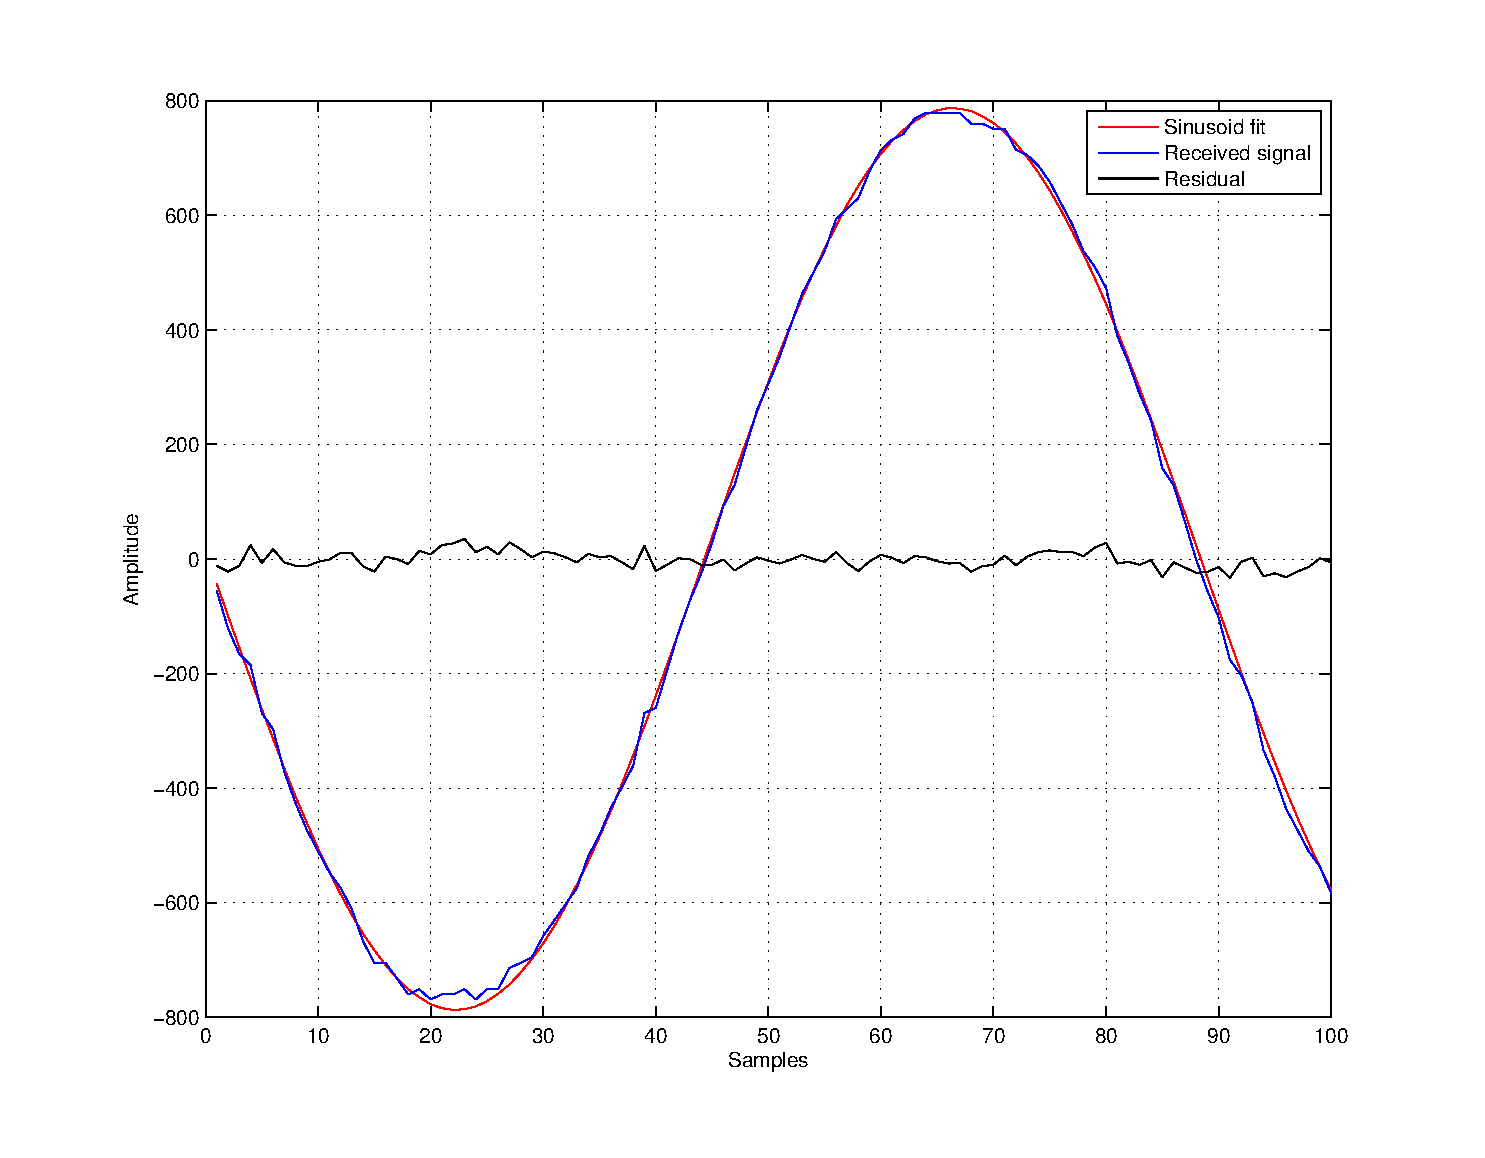
\includegraphics[width=0.7\textwidth]{sinusoid_fit.eps}
    \caption[BFSK example]{Example of a received sinusoid with frequency of 500 Hz together with sinusoid fit.}
    \label{fig:sinusoid_fit}
\end{figure}

For any channel there is a maximum achievable rate called the channel capacity. In the case of a real valued AWGN channel with bandwidth \(W\) this capacity can be shown to be

\textcolor{red}{Do we need a reference for this?}%

\begin{equation}\label{Eq:awgn_capacity} C = \frac{W}{2}\log_2(1+\text{SNR})\text{                [bits/s]}\end{equation}



\section{Signal-to-Noise Ratio Measurements}

Both measurement methods were evaluated on received signals of length \(N = 44.1\times10^4\) samples corresponding to a signal of \(10\) seconds. For the SINAD measurement a sinusoid with frequency \(11025\) Hz \((F_s/4)\) was used. The histogram of the residual noise in the SINAD measurement can be seen in Figure \ref{fig:noise_histogram}. This figure show that the noise have a distribution of Gaussian character. The resulting values of SNR and SINAD measurements can be seen in \ref{table:snr}.


\begin{table} [h]
\centering
\begin{tabular}{lcccc} 
\bf{Method}	& \bf{Measured value }\textnormal{[dB]}    & \bf{AWGN capacity}\textnormal{[kbps]} \\
\hline
\emph{SNR}           & 51.19           & 218       \\
\emph{SINAD}        & 29.71           & 375           \\
\end{tabular}
\caption[Result of signal-to-noise ratio measurements]{Results of measurements of SNR with the two different approaches together with the resulting channel capacity.}
\label{table:snr}
\end{table}


\begin{figure}[H]
  \centering
    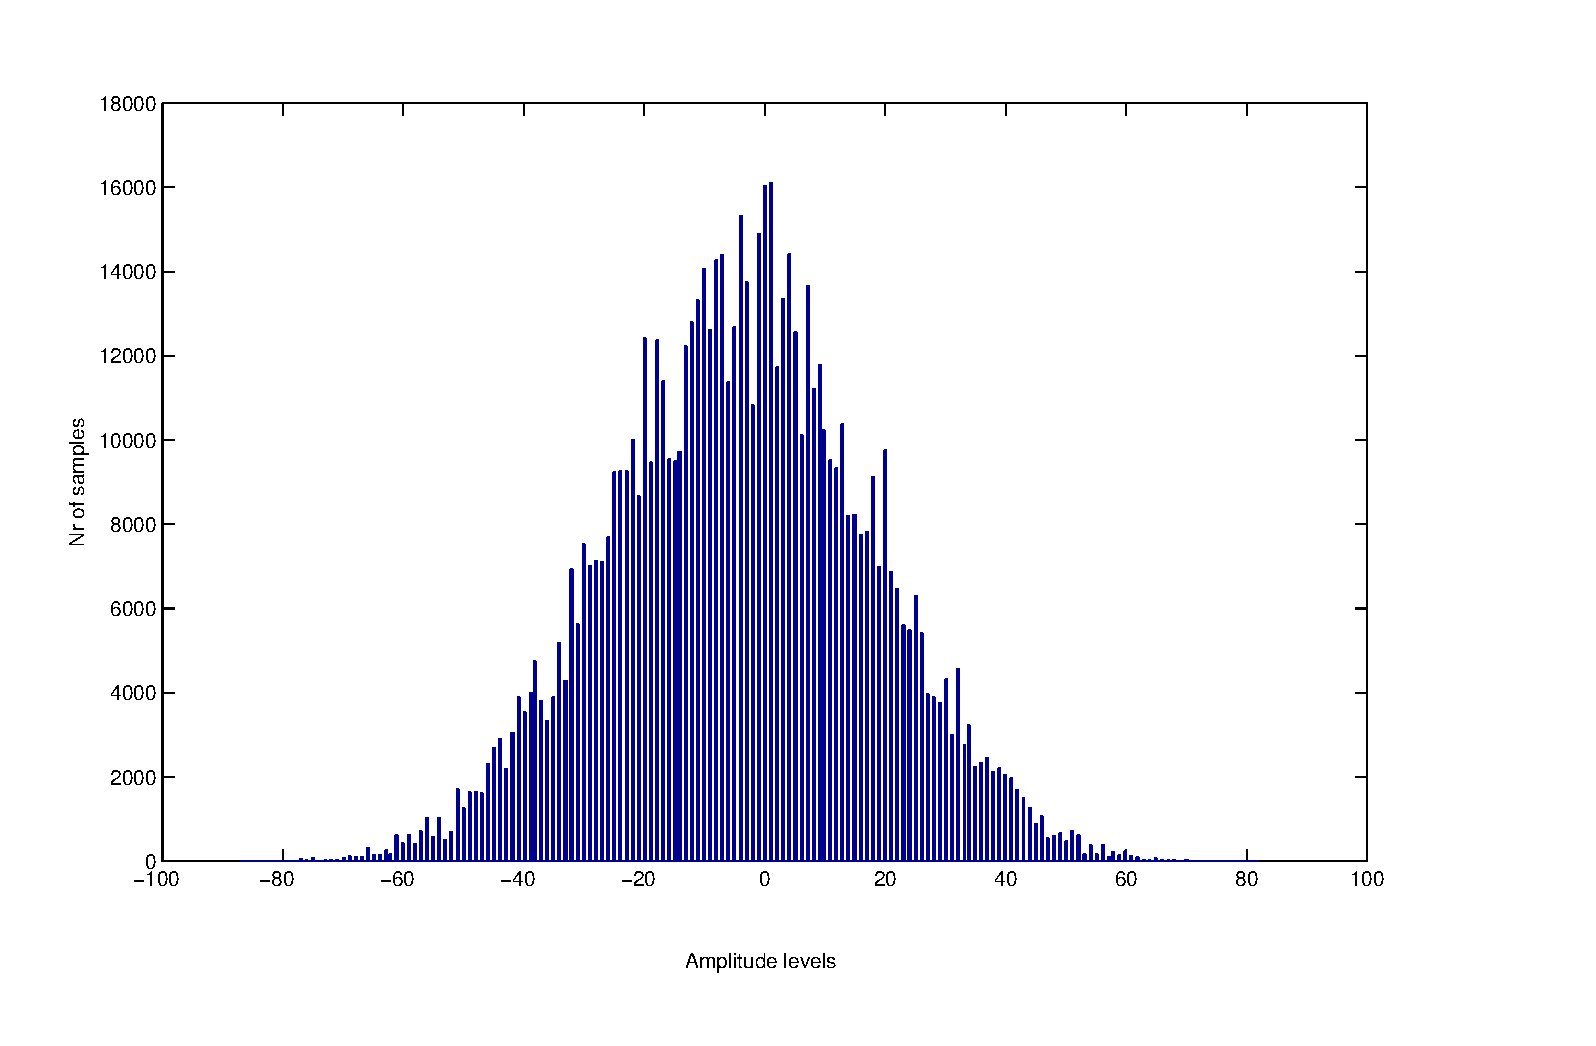
\includegraphics[width=0.7\textwidth]{snr_noise_histogram.eps}
    \caption[BFSK example]{Histogram of residual noise on transmitted sinusoid in SINAD measurement.}
    \label{fig:noise_histogram}
\end{figure}

\section{4-FSK}

In the implementation, 35 samples per symbol and the frequencies \(kF_s/24\) for \(k=1,4,7,10\) were used. This resulted in a rate of 
2520 bps with no errors.  This value for the rate considers all the bits that were transmitted, including guard band and training sequence in total consisting of 400 bits. Hence, the effective rate is lower than this value but still well above the basic requirements of 1 kbps. 
In Figure \ref{fig:4FSKspectrum} plots of the transmitted spectrum is shown with rectangular and Gaussian window. 

\begin{figure}[H]
  \centering
    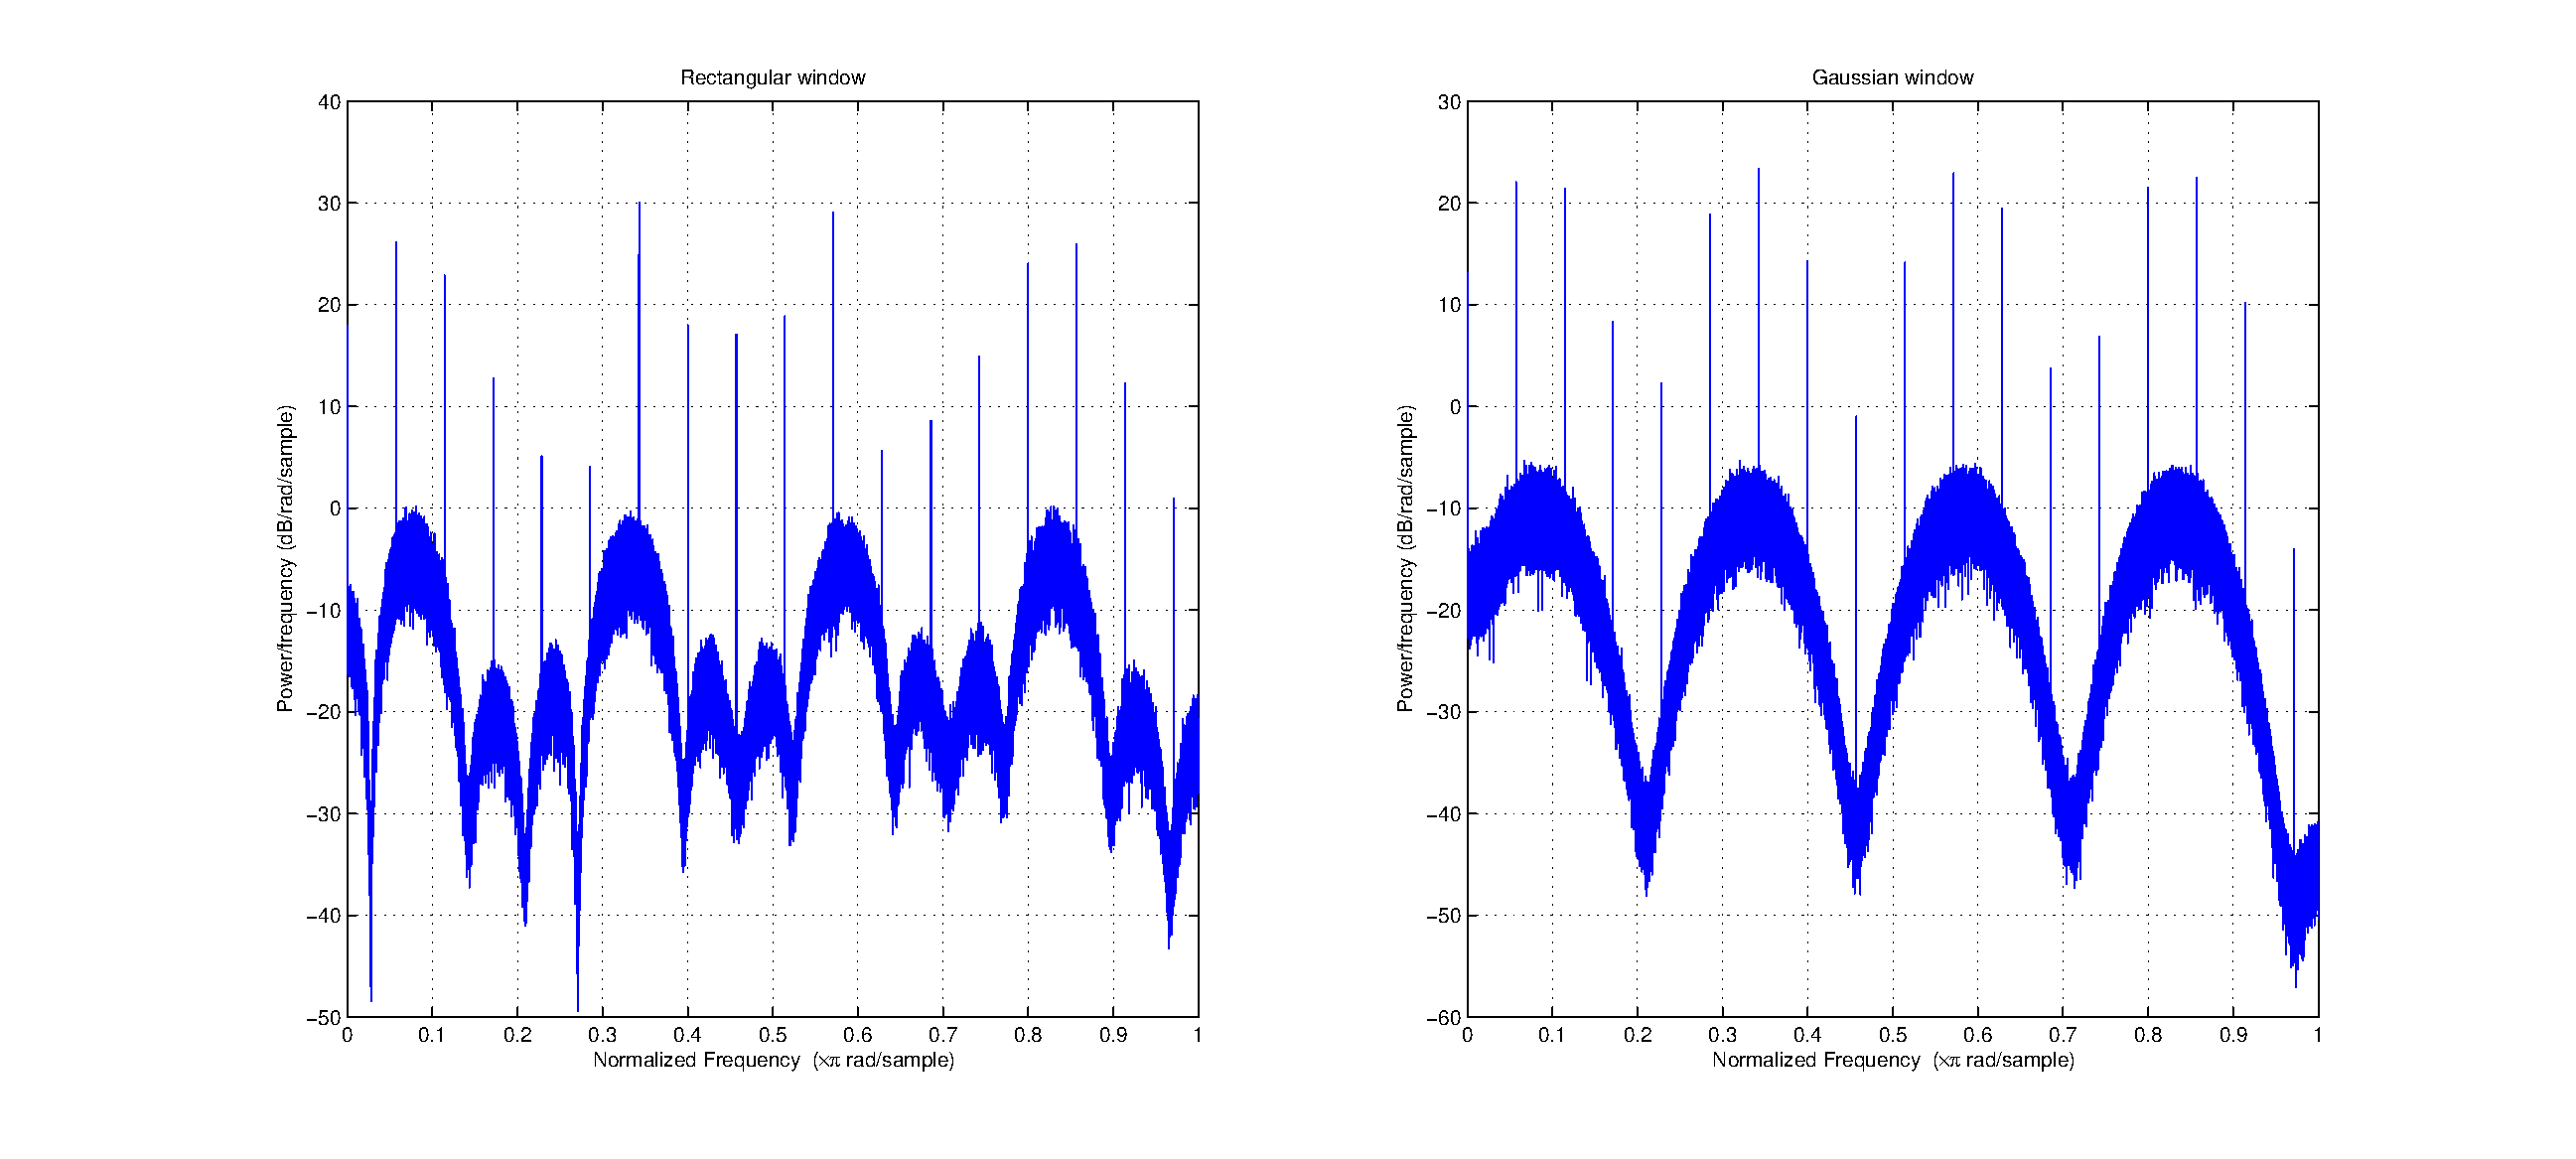
\includegraphics[width=1.0\textwidth]{4FSKspectrum_windoweffect.eps}
    \caption[4-FSK spectrum]{Spectrum of the transmitted 4-FSK signals with rectangular and gaussian window.}
    \label{fig:4FSKspectrum}
\end{figure}

In order to improve the rate and more efficiently exploit all the available bandwidth, a frequency division multiplexing (FDM) system was used. The idea is to put the frequencies in the 4-FSK scheme closer together and divide the spectrum into \(N_r\) parallel channels. \(N_r = 7\) was the highest number of channels that the system could demodulate reliably i.e 0 \% BER. However, it was necessary to lower the rate by increasing \(n_{sym}\) to 88 samples per symbol. The resulting rate was

$$ R = \frac{N_r\times log_2(4)}{n_{sym}}\times f_s = 7 \times \frac{2}{88}\times f_s =7015 \text{ bps}$$


Hence, this approach more than doubles the rate that was achieved with the single 4-FSK system. A Gaussian pulse shape was used to reduce the interference between frequencies close to each other. We tested the system to find the minimum number of samples per symbol needed for 0 \% BER with \(N_r=2,4,7\).
The results can be found in Table \ref{table:FDM}. The transmitted power spectrum for the case \(N_r= 4\) is depicted in Figure \ref{fig:4FSKFDM}.

\begin{table} [h]
\centering
\begin{tabular}{lcccc} 
\(N_r\)	&  Samples per symbol  & Rate \textnormal{[bps]} \\
\hline
\emph{2}           & 37          & 4767       \\
\emph{4}        & 63           & 5600           \\
\emph{7}        & 88           & 7015           \\
\end{tabular}
\caption[Result of 4-FSK + FDM]{4-FSK + FDM results for different values of \(N_r\)}
\label{table:FDM}
\end{table}


\begin{figure}[H]
  \centering
    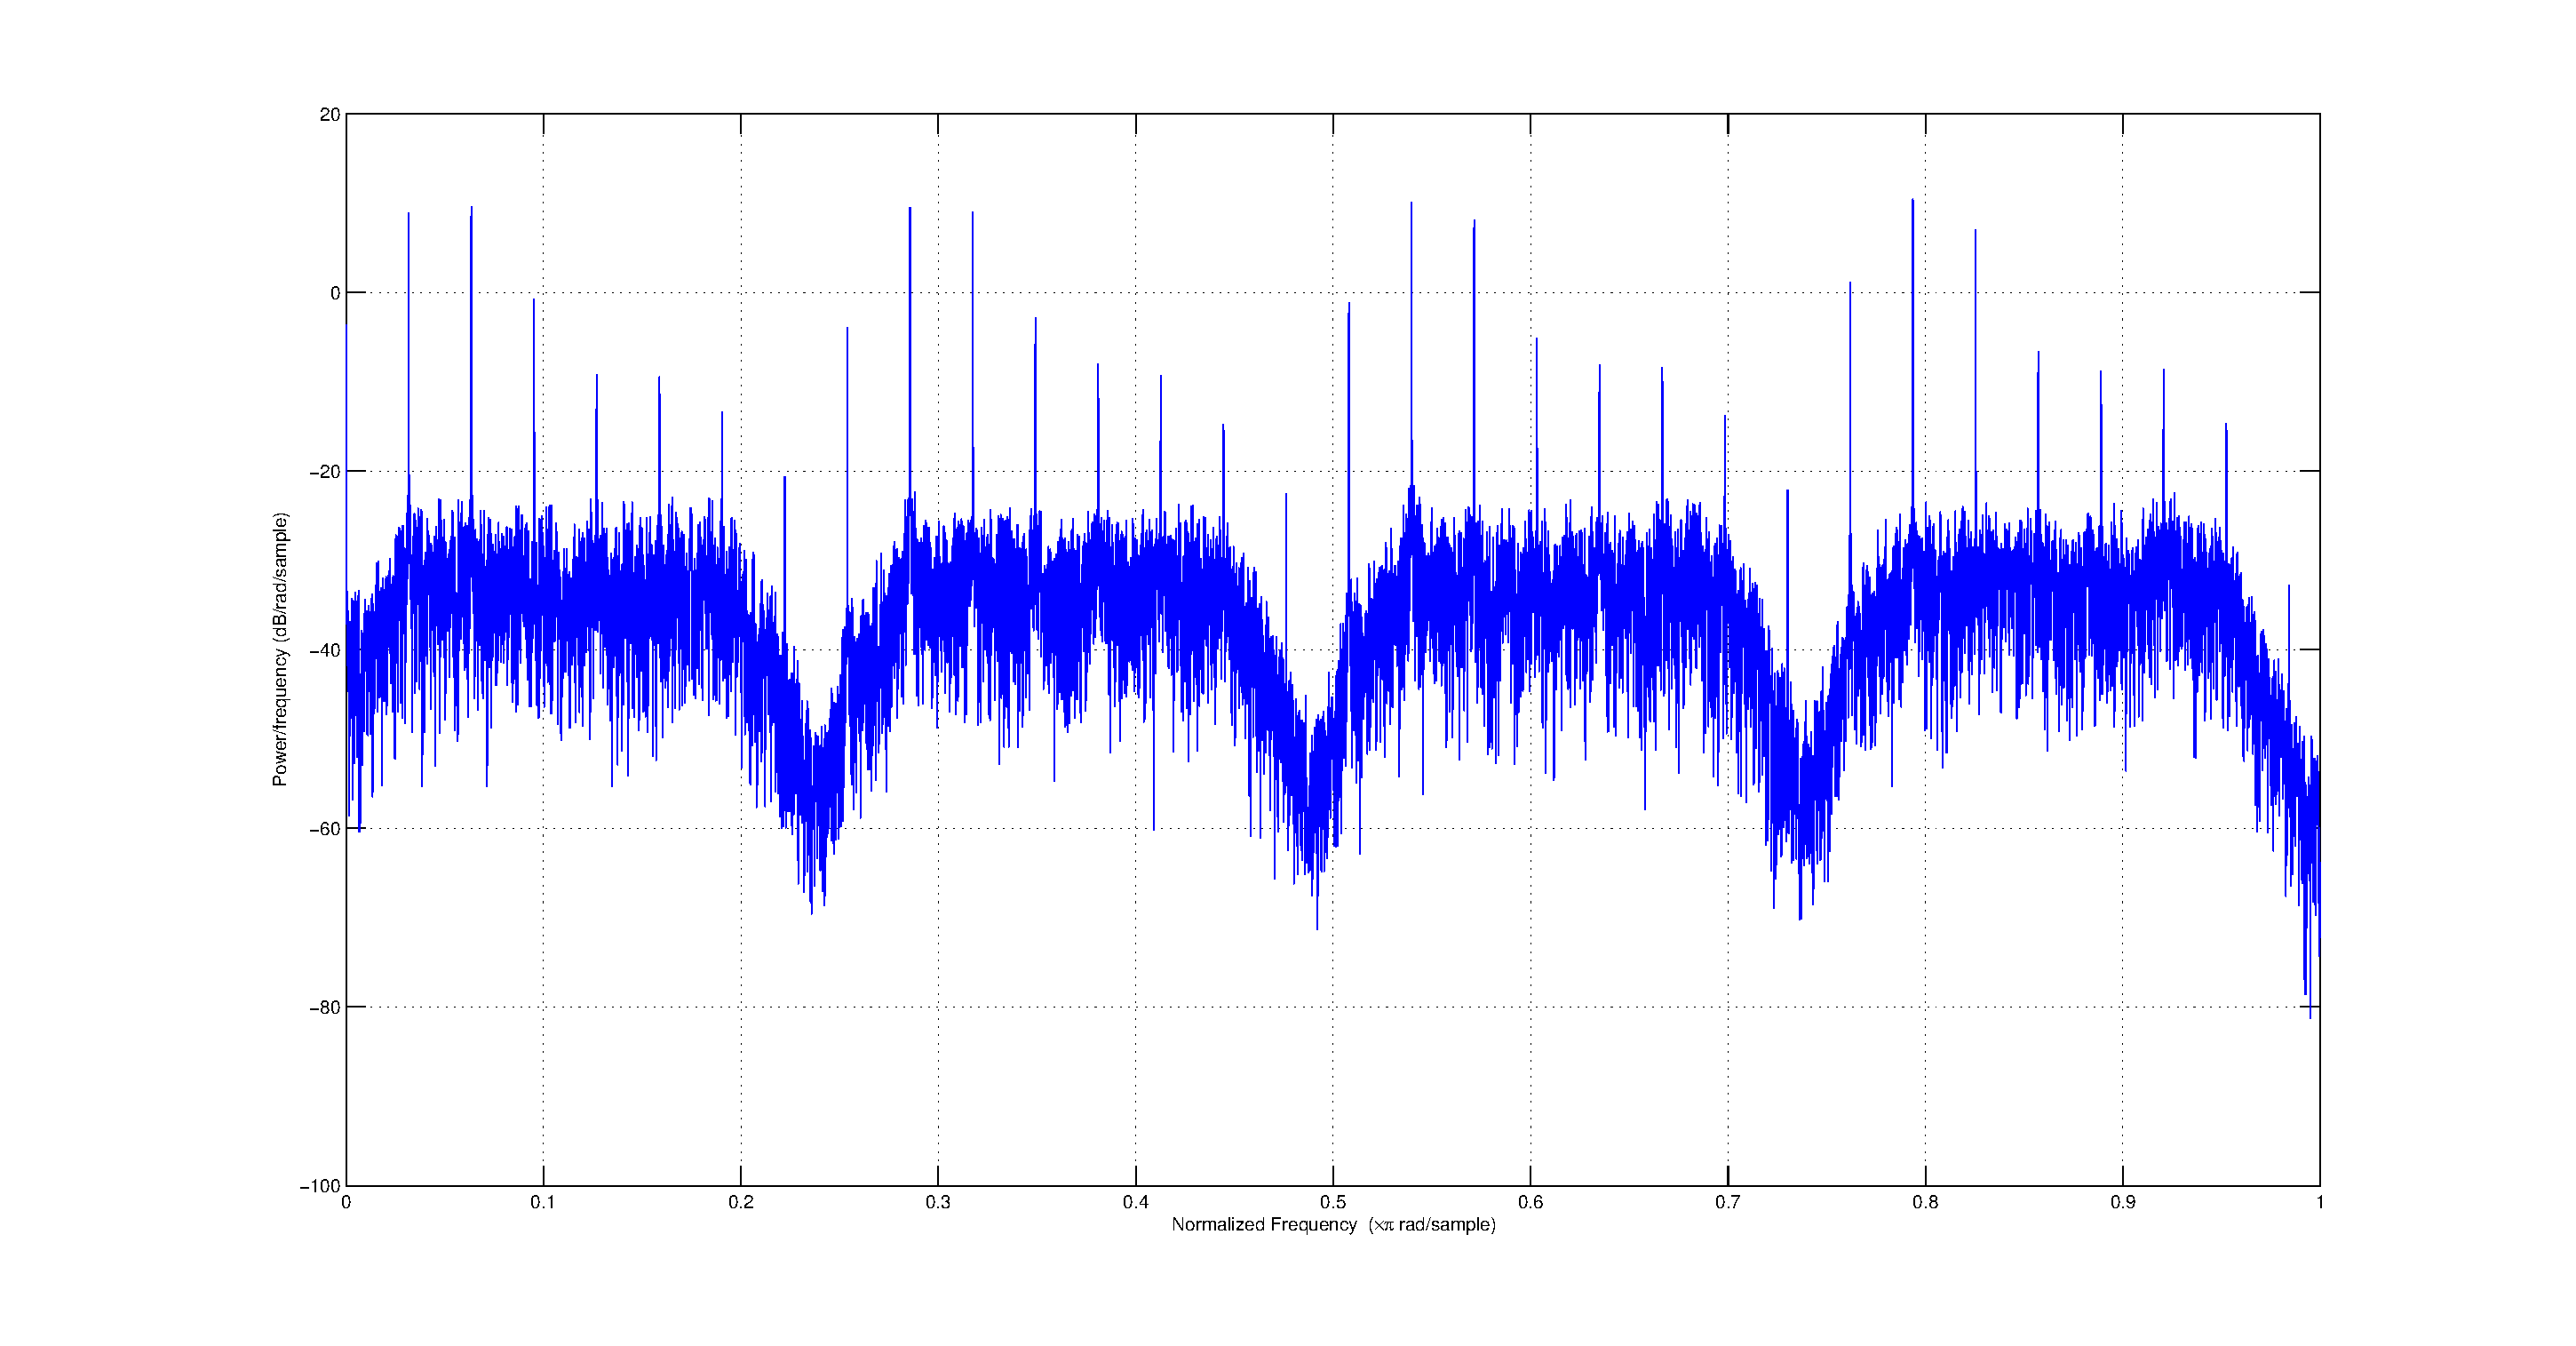
\includegraphics[width=1.0\textwidth]{4FDMspectrum.eps}
    \caption[4-FSK spectrum]{Spectrum of the 4-FSK signal extended to 4 FDM.}
    \label{fig:4FSKFDM}
\end{figure}
\section{M-QAM}

In this implementation we found the best performance with 64-QAM and 8 samples per symbol. We used a carrier frequency of 11025 Hz and a Gaussian pulse shape for the modulation which gave us an effective rate of 28.6 kbps when transmitting a file of 10 kB. The power spectrum of the transmitted signal and the received constellation is shown in Figures \ref{fig:qam_spectrum} and \ref{fig:64qam_constellation}. Reducing the number of samples per symbol to 7 widens the main lobe of the signal such that its bandwidth exceeds the bandwidth of the system. This and possibly the effect of ISI made it impossible to demodulate such a signal without getting errors.

\begin{figure}[H]
  \centering
    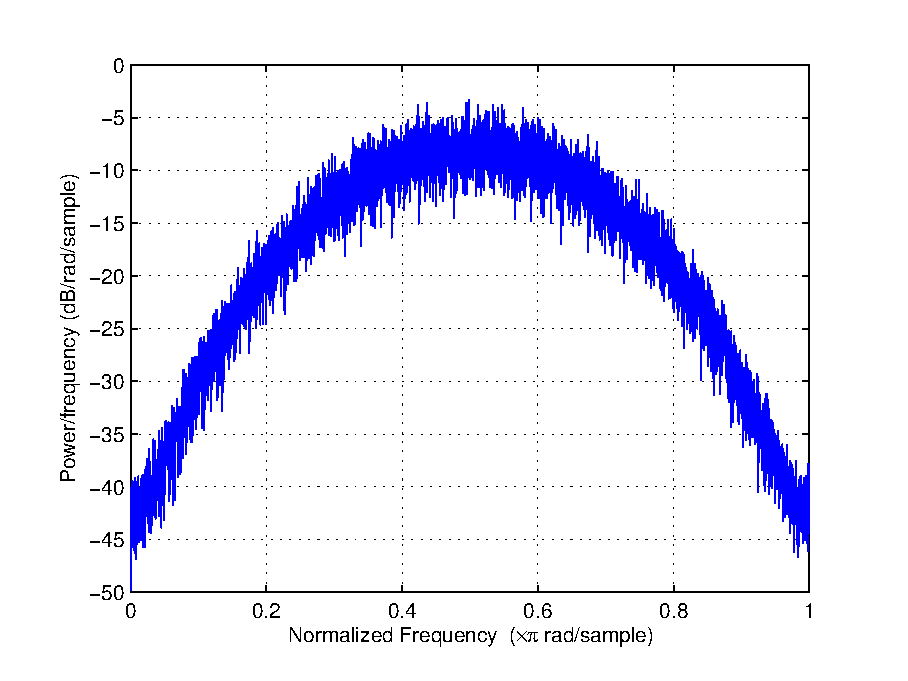
\includegraphics[width=0.7\textwidth]{64QAMspectrum.eps}
    \caption[64-QAM spectrum]{Power spectrum of the transmitted 64-QAM signal with gaussian window.}
    \label{fig:qam_spectrum}
\end{figure}

\begin{figure}[H]
  \centering
    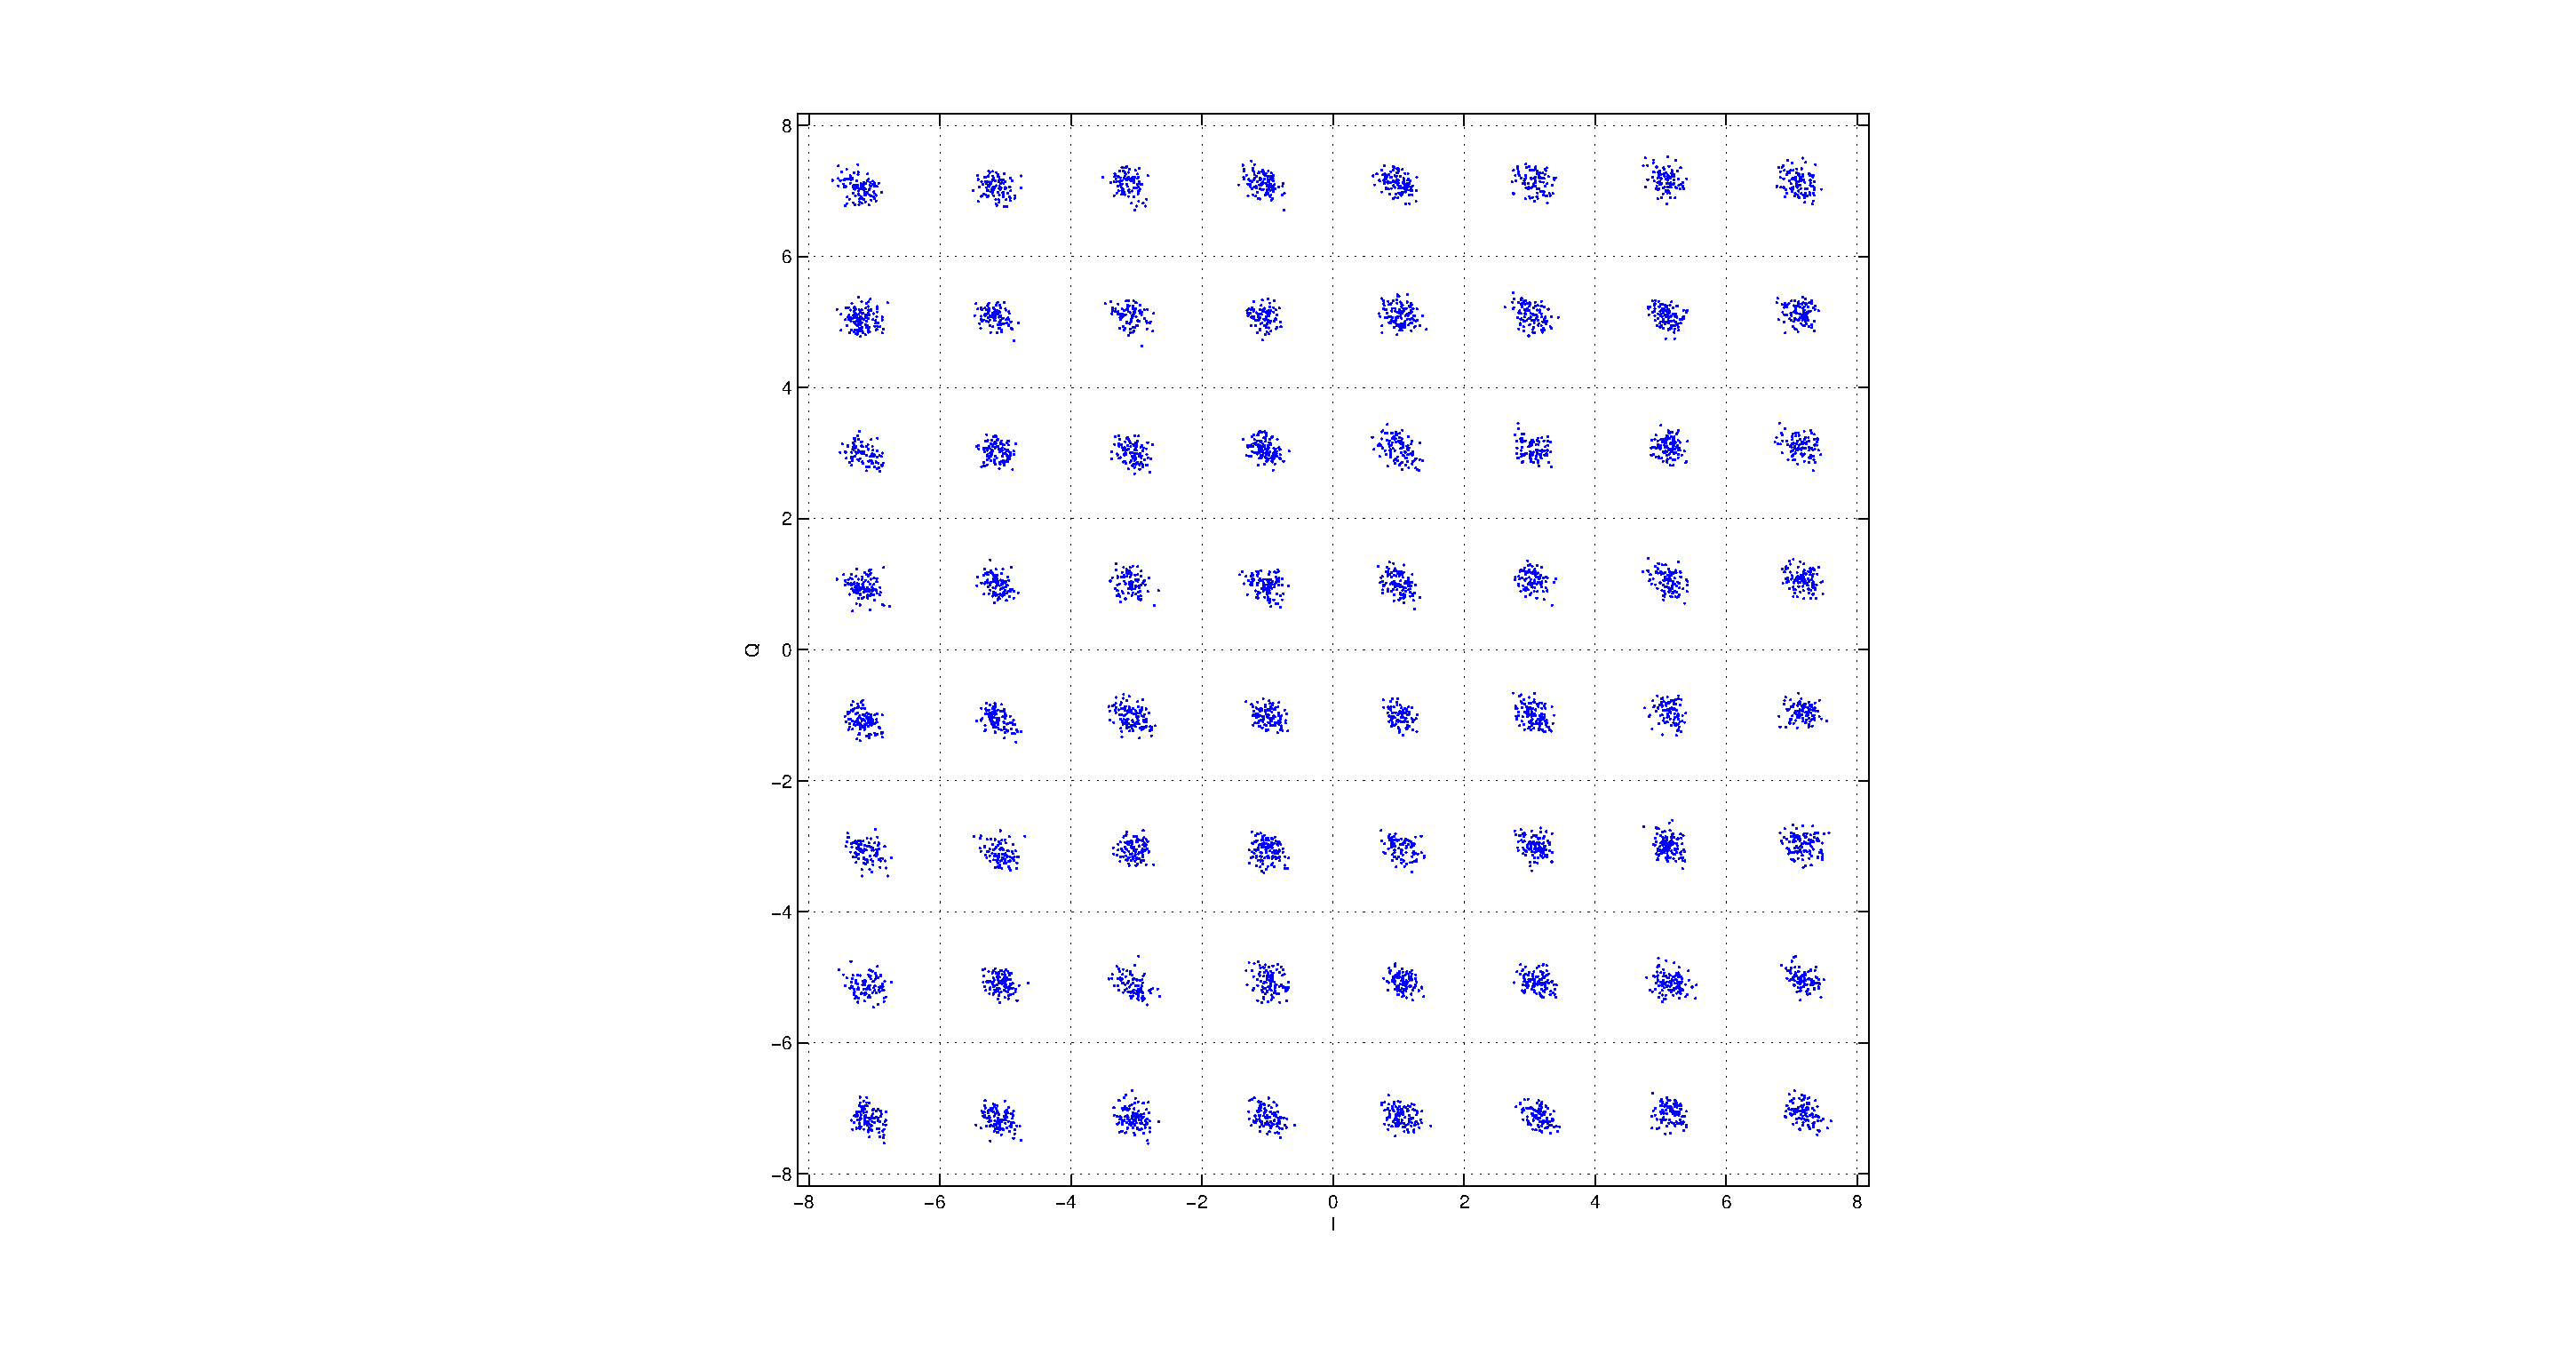
\includegraphics[width=1.0\textwidth]{64QAMscatter.eps}
    \caption[64-QAM constellation]{Received constellation after offline transmission with 64 QAM.}
    \label{fig:64qam_constellation}
\end{figure}




\begin{thebibliography}{1}

\bibitem{Madhow}
Madhow U., \emph{Fundamentals of Digital Communication}, Cambridge , 2008.

\bibitem{Proakis}
Proakis J. ,Salehi Masoud, \emph{Digital Communications}, McGraw-Hill , 2008.

\bibitem{ASKDemGaza}
Abu M., \href{http://site.iugaza.edu.ps/mabufoul/files/2010/09/Experiment-5.pdf}
{\emph{ASK demodulator Lab Experiment}},
Islamic University of Gaza, retrieved in April 2014.


\bibitem{DigModTech}
Sa-nguankotchakorn T. , \href{http://www.tc.ait.ac.th/faculty/teerapat/AT77.11_Digital\%20Modulation\%20Techniques/III.Frequency_Shift_Keying.pdf}{\emph{Frequency Shift Keying Lecture Slides}}, Asian Institute of Technology, retrieved in April 2014.


\bibitem{DigCommLec}
Okechukwu C. Ugweje, \href{ugweje/web/Courses/Ee549/Handout/EE549F01Lecture37.pdf}{\emph{Frequency Shift Keying, Lecture Slides}},  University of Akron, retrieved in April 2014.


\bibitem{XiongDigModTech}
Xiong F., \emph{Digital Modulation Techniques}, Artech House, 2006.

\bibitem{gold}
Shembil S., \emph{M-Ary FSK with Orthogonal Pulse Envelopes and its Noncoherent Detection}, IJECS-IJENS, Vol. 10, No.06, Issued December 2010, pp. 103-106.

\bibitem{GoertzelPaper}
Sysel and Rajmic, \emph{Goertzel algorithm generalized to non-integer multiples of fundamental frequency}, EURASIP Journal on Advances in Signal Processing, 2012, 2012:56.

\bibitem{ProjectEQ2310}
Project Assignment EQ2310 Digital Communications, \emph{Analysis and Simulation of a QPSK System}, KTH, 2013.

\bibitem{EQ2440ProjectDescription}
Project Description EQ2320 PROJECT IN WIRELESS COMMUNICATION, \emph{Project \#1: In-flight file-transfer using 3-mm cable}, KTH, 2014.

\bibitem{HaykinBook}
Haykin S., \emph{Digital Communication Systems}, John Wiley \& Sons, Inc., 2014.

\bibitem{CarrierSynchPaper}
Dick D., Harris F., and Rice M., \emph{FPGA Implementation of Carrier Synchronization for QAM Receivers}, Journal of VLSI Signal Processing 36, 57-71, 2004.

\bibitem{NI QAM white-paper}
National Instruments, (2012),\href{http://www.ni.com/white-paper/3896/en/}{\emph{Quadrature Amplitude Modulation (QAM)[White paper]}}, retrieved in May 2014.

\bibitem{Agilent IQ paper}
Agilent Technologies,(2013) \href{http://wireless.agilent.com/wireless/helpfiles/89600B/WebHelp/subsystems/digdemod/content/digdemod_para_interact_iqgainimb_quadskewerr.htm}{\emph{IQ Gain Imbalance and Quadrature Skew Error Data Interaction (Digital Demod)[9600 VSA Software - Product Documentation]}}, retrieved in May 2014.

\bibitem{BER-QAM paper}
Yoon D., Cho K., and Lee J., \emph{Bit Error Probability of M-ary Quadrature Amplitude Modulation}, Vehicular Technology Conference, 2000. IEEE-VTS Fall VTC 2000. 52nd , vol.5, no., pp.2422,2427 vol.5, 2000.
\bibitem{DSPDiniz}
Diniz P., Da Silva E., Netto S., \emph{Digital Signal Processing: System Analysis and Design}, Cambridge University Press, 2010.

\bibitem{SklarBook}
Sklar B., \emph{Digital Communications Fundamentals and Applications}, Prentice Hall, 2001.


\bibitem{FFTJavaRef} 
Robert Sedgewick and Kevin Wayne,
\href{http://introcs.cs.princeton.edu/java/97data/FFT.java.html}{\emph{FFT.java}},  Princeton
Copyright © 2000–2011

\bibitem{ComplexJavaRef} 
Robert Sedgewick and Kevin Wayne,
\href{http://introcs.cs.princeton.edu/java/97data/Complex.java.html}{\emph{Complex.java}},  Princeton
Copyright © 2000–2011



%% Slides & handouts



\end{thebibliography}


\end{document}